\documentclass{assignment-263}

\anum{4}
\course{CSC263}
\duedate{Mar. 27, 2025}
\filename{ps4.pdf, ps4.tex, ps4.py}

\usetikzlibrary{automata, positioning, arrows}

\begin{document}
\think
\begin{enumerate}
\item \textbf{[12 points]}
	You are given a weighted, connected, undirected graph $G=(V, E)$ and
    one of its minimum spanning trees $T\subseteq E$. Furthermore, you are guaranteed that the edge weights are all distinct.

    \begin{enumerate}
      \item \textbf{[6 points]}
        A new edge $(u, v)$ with weight $w_{u, v}\;(u, v\in V)$ is
        added to $G$, resulting in a new graph $G'=(V, E\cup \{(u,
        v)\})$. How do you efficiently find a minimum spanning tree
        $T'$ of $G'$? Describe and justify your algorithm in concise
        and precise English, and analyse its runtime. To get full
        marks, your algorithm's worst-case runtime must be in
        $\mathcal{O}(|V|)$.

      The algorithm works as follows. First, add the new edge \((u,v)\) to \(T\). Since \(T\) now has \(n\) edges and \(n\) vertices, it is guaranteed to contain some loop. We perform a DFS starting at \(u\) to find this loop, and we know it is successful when the algorithm encounters \(u\) again. Finally, iterate through the edges contained in this loop and remove the edge with the highest weight. This new tree is guaranteed to be the a minimum spanning tree of \(G'\).

      Now, we will show that this algorithm has a worst-case runtime of \(\mathcal{O} (|V|)\). Adding the new edge to \(T\) takes constant runtime, so that is not our main point of concern. The DFS on \(T\) has a worst-case runtime of \(\mathcal{O} (|V| + |E|) = \mathcal{O} (|V|)\), and we might need to iterate through every edge, if the loop in the graph contains every edge, which has a runtime of \(\mathcal{O} (|T|) = \mathcal{O} (|V|)\). Thus the worst-case runtime of this algorithm is \(\mathcal{O} (|V|)\).

      \item \textbf{[4 points]} Prove that the second lightest edge in the graph should belong to every minimum spanning tree.
      
      Suppose for contradiction that there exists a minimum spanning tree that does not contain the second lightest edge. Assume that this edge connects some vertices \(u,v\). It must be true that there is some path in the minimum spanning tree \(T\) that connects \(u\) and \(v\). We make the assumption that \(G\) is simple (so there is not another edge directly connecting \(u,v\)), implying that this path traverses at least \(2\) edges. Of these edges, there is guaranteed to be one edge \((r,s)\) that is strictly heavier than \((u,v)\). Create a new subgraph which contains all the edges of \(T\), but contains the edge \((u,v)\) and excludes the edge \((r,s)\). Notice that this subgraph is a spanning tree whose total edge weight is less than \(T\), which contradicts the fact that \(T\) is a minimum spanning tree. Therefore all minimum spanning trees should contain the second lightest edge.
      
      \item \textbf{[2 points]} Prove that the third lightest edge in the graph may not be in a minimum spanning tree.
      
      Consider the graph
      \begin{center}
        \centering
        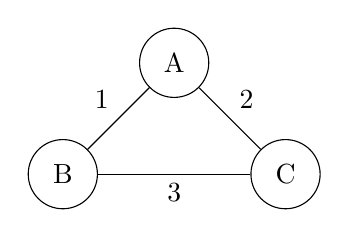
\begin{tikzpicture}[node distance=2cm]
          \node[state] (A) {A};
          \node[state,below left of=A] (B) {B};
          \node[state,below right of=A] (C) {C};
          \path (A) edge [] node[above left] {1} (B);
          \path (A) edge [] node[above right] {2} (C);
          \path (B) edge [] node[below] {3} (C);
        \end{tikzpicture}
      \end{center}
      It is quite clear that the only minimum spanning tree for this graph is the subgraph obtained by removing the edge with weight 3. But this edge is also the third lightest edge, which illustrates what we wanted.
    \end{enumerate}

	\end{enumerate}

  \begin{enumerate}
    \item[2.] \textbf{[6 points]}
    You are given a $k \times k$ grid of squares (think of a chess board). Each square is identified by $(i,j) \in [k] \times [k]$ where $[k] = \{1,2,...,k\}$, $i$ is the row number, and $j$ is the column number. From any square you are allowed to make one of the following moves: (i) $m$ steps in the vertical direction and $n$ steps in the horizontal direction, or (ii) $n$ steps in the vertical direction and $m$ steps in the horizontal direction. If you encounter the edge of the board (either a vertical edge or a horizontal edge) while making the move, then the move is invalid. For example, if $m = 1$ and $n = 2$, then this corresponds to the moves made by the knight on a chess board. You play this game with your friend. Your friend first chooses a square $(i,j) \in [k]\times [k]$. Your task is to find another square $(i',j') \in [k] \times [k]$ such that there is no valid sequence of moves from $(i,j)$ to $(i',j')$, or declare that no such $(i',j')$ exists. Devise an $O(k^2)$ algorithm to solve this task.
 \end{enumerate}

 \textbf{Solution:} Our algorithm works as follows. First, we treat the grid as a graph, where each square is a vertex, and
 \[
  ((i,j), (i - n, j - m)),((i,j), (i - n, j + m)),((i,j), (i + n, j - m)),((i,j), (i + n, j + m))
 \]
 are edges, if the squares are in \([k]\times [k]\). Notice that in this graph, there are \(k^2\) vertices and at most \(4k^2\) edges. We perform a DFS on this graph originating from the original square chosen, which we call \((i,j)\). This has a run time of \(\mathcal{O} (k^2)\). Afterwards, we iterate through each vertex with a nested for loop. If we find a vertex \((i', j')\) that has not been visited, that implies that it cannot be reached from \((i,j)\), so we return that square. If we completely iterate through the grid without finding an unvisited square, then that means all squares are reachable, so no square is unreachable.

\program

\begin{enumerate}
\item[3.] \textbf{(12 points)}
  You are planning an around-the-world trip with your two best friends for the summer. 
There is a total of $n$ cities that the three of you want to visit.
As you are traveling around the world, you are worried about time zones and airport access. Therefore, some cities can only be visited after visiting another city first, which is in a nearby timezone or has an airport, which are expressed as a list of pairs (cityX,cityY) (cityX can only be visited after visiting cityY).

Given the total number of cities and a list of dependency pairs, is it possible for you all to visit all cities?

Your task is to write the function \verb|can_visit_all_cities|, which determines whether visiting the $n$ cities is possible or not given the dependencies. \textbf{(8 points)}

\textbf{Requirements}
\begin{itemize}
\item Your code must be written in Python 3, and the filename must be \verb|ps4.py|.
\item We will grade only the \verb|can_visit_all_cities| function; please do not change its signature in the starter code. include as many helper functions as you wish.
\item You are {\bf not} allowed to use the built-in Python dictionary or set.
\item To get full marks, your algorithm must have average-case runtime
  ${O}(m + n),$ where $m$ is the number of dependencies given.
\end{itemize}

\textbf{Input/Output Specification}
Please see the python starter code for input / output
specifications. 

\textbf{Write-up (4 points)}: in your \verb|ps4.pdf/ps4.tex| files,
include the following: an explanation of how your code works,
justification of correctness, and justification of desired
${O}(m + n)$ average-case runtime.

This algorithm works by converting the list of dependencies into a graph, and then using DFS to find cycles. It makes use of the fact that all cities are reachable if and only if the graph does not contain any cycles. To see this, suppose that the graph has a cycle. This means that there are two cities that indirectly depend on each other (i.e. a city depends on another city that eventually depends on the other city), which means that it is impossible to visit either of those cities. Now, suppose that there are no cycles in the graph. Each chain of dependencies must terminate. Using an inductive argument, we can argue that the dependecies of any city are reachable, therefore making every city reachable.

As for the implementationg, the algorithm first converts the list of dependencies into a directed graph, by using a hash table with capacity \(2n\) that stores each city name as a key and the list of cities that have the key as a dependency for the value. The algorithm performs a DFS to find a cycle. In particular, it marks each city as either not visited, visiting, or visited as it traverses the graph, and if it encounters a city that has "visiting" status, it knows that a cycle has been found. If a cycle has been found, not every city is reachable, so the algorithm returns false. Otherwise, return true.

To compute the average case runtime, we assume that each combination of dependencies is equally likely and further assume that our hash table possesses the uniform hashing property. Let \(n\) be the number of cities and let \(m\) be the number of cities. Converting the list of dependencies into a graph requires iterating through each edge and inserting it into the hash table. Since we assume the uniform hashing property, and the load factor less than one, each insertion takes constant time, so constructing the graph takes \(O(m)\). Finally, the DFS has a runtime in \(O(n+m)\), no matter how the edges are distributed. Thus the total average case runtime is \(O(n+m)\).

\end{enumerate}

\end{document}

%%% Local Variables:
%%% mode: latex
%%% TeX-master: t
%%% End:
